\section{Defining and Instantiating a Benchmark for Insight Anticipation}
\label{sec:dataset_construction}

\paragraph{Task Definition.} We introduce the setting of insight anticipation: given an input context with two paper summaries $x = (x_A, x_B)$ where $x_A$ is a summary of paper $A$, and $x_B$ is a summary of paper $B$, the goal is to generate the key insight of a downstream paper that builds on $A$ and $B$. We denote this ground truth downstream insight statement as $y^*$. $y^*$ is an oracle insight that emerges only when both papers are considered together. This task requires the model to consider how $A$ and $B$ might jointly influence a downstream paper and generate a research insight/idea $\hat{y}$ that is semantically similar to $y^*$. This setup intentionally restricts the number of parents to two (as more papers lead to context management constraints for training and inference), making the task a conservative lower bound on the full problem. We do not address parent discovery, focusing instead on whether meaningful insight synthesis is possible given fixed inputs. Figure~\ref{fig:insight_generation_prompt} shows the insight generation prompt we use for training or evaluating all models. 


\paragraph{Dataset Construction.}
We create a dataset $\{((x_A, x_B)_i, y^*_i)\}_{i=1}^N$ as follows. We collect $17{,}839$ papers from arXiv that are published between May 23rd, 2007, and January 23rd, 2026, according to their latest update date on arXiv. Since arXiv is not peer reviewed, the raw corpus may contain noisy or non-substantive documents. To mitigate this, we retain only papers with at least two citations.\footnote{We use citation counts from Semantic Scholar as a proxy for paper quality.} We download these papers as a PDF. For each paper, we prompt \gemtwoflash{}
% \footnote{\href{https://docs.cloud.google.com/vertex-ai/generative-ai/docs/models/gemini/2-5-flash}{https://docs.cloud.google.com/vertex-ai/generative-ai/docs/models/gemini/2-5-flash}}
to identify two prior papers that this paper explicitly cites and builds upon by combining their ideas in a synergistic way. We also ask \gemtwoflash{} to explain the synergy (see the full prompt in Figure~\ref{fig:upstream_citation_prompt}). We then download the two parent papers as a PDF and use their content as input context $x$. Ideally, we would like to take the full paper content as input to the model and ask it to generate a downstream insight. However, given the context-length limitations of existing LMs as well as the high inference cost, we instead opt to prompt \gemtwoflash{} to summarize the paper. We then use paper summaries as the input. 
We use the following prompt to summarize each paper into key insights and contributions: ``\textit{Summarize the document, clearly describing the method used and highlighting the key insights or findings. Provide sufficient detail so that the approach and main contributions are fully understood.}'' 
For $y^*$, we use the synergy explanation that is part of the output to the parent-identification prompt in Figure~\ref{fig:upstream_citation_prompt}). 
% This next sentence is a bit unclear in terms of what explanation you are referring to. Could be useful to reword.
We cannot use the raw explanation because it refers to a future downstream paper and talks about the insight in the context of the two parent papers. Instead, we would like the model to generate a standalone insight statement directly from the two parent papers alone. Therefore, we prompt \gemthreepro{} to rewrite the insight and explanation without reference to the downstream paper (see prompt in Appendix~\ref{appendix:rewriting_insight_prompt}). After constructing all $(x,y^*)$ pairs, for each unique pair of parent papers $x=(x_A, x_B)$, we keep the insight $y^*$ from the most cited downstream paper in order to prioritize generating more impactful insights.

% TODO: Figure out location for this
\begin{wrapfigure}{r}{0.4\textwidth}
    \centering
    \vspace{-8mm}
    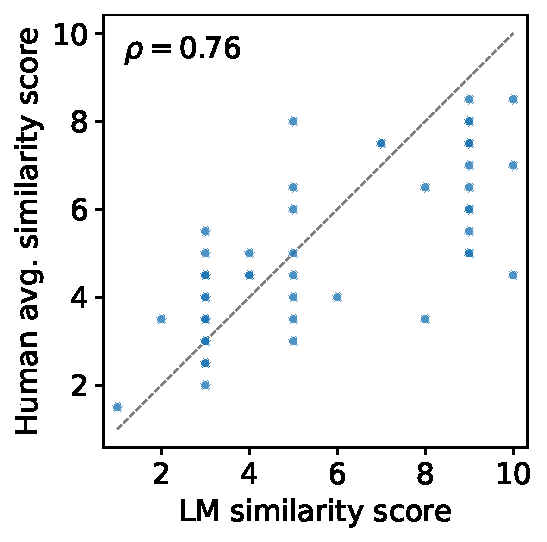
\includegraphics[width=0.9\linewidth]{figs/lm_vs_human_scatterplot.pdf}
    \caption{\footnotesize \textbf{Human experts align with LM judge.} LM similarity scores are positively correlated with human similarity scores (Spearman $\rho = 0.761$, $p < 0.001$, $n = 60$).}
    \label{fig:lm_vs_human_scatterplot}
    \vspace{-0.5cm}
\end{wrapfigure}
\paragraph{Temporal Hold-Out Evaluation.}
To more rigorously assess generalization, we conduct all evaluations on a \emph{future held-out test set} consisting of downstream papers published after the training cutoff date. We split the dataset by the publication date of the downstream paper in each $(x, y^*)$ pair. Papers published before July 1st, 2023 are used for training. To study the ability of models to generalize to new domains, we restrict the training set to papers tagged with cs.CL (Computation and Language), yielding $N=10{,}335$ training examples. For evaluation, we consider papers published after July 1, 2023 and randomly sample up to $600$ papers from each domain (see the category taxonomy in Appendix~\ref{appendix:domain_mapping}), resulting in a test set of $7{,}504$ papers. No papers from this test set are seen during training, though some of them may share at most 1 parent paper with the papers in the training set. We also conduct evaluations on a subset of the test set that does not have any overlapping parents with those in the training set. We call the subset \textbf{Test-unseen-parents} ($N=5{,}294$).

\paragraph{Evaluation Metric.}
For each generation, we prompt an LM judge to give a \textbf{similarity score} ranging from 1 to 10 (higher is better) comparing the model-generated insight to the ground-truth insight $y^*$. We use \gemthreepro{} as the judge model (see Figure~\ref{fig:similarity_judge_prompt} for the prompt). To assess the reliability of the LM-based evaluation, we conduct a human evaluation study on $30$ pairs of insights generated by \qwenfourb{} and \ourmethod{} ($n = 60$). Two human annotators, who are PhD students in Computer Science, independently rate the similarity between model-generated insights and ground-truth insights using the same rating scale as the LM judge. The LM’s scores show a statistically significant positive correlation with the average scores across human annotators (Figure~\ref{fig:lm_vs_human_scatterplot}). In particular, we observe a Spearman rank correlation of $\rho = 0.761$ ($p < 0.001$). More details can be found in Appendix~\ref{app:human_eval}.

\begin{AIbox}{Takeaways of Insight Anticipation Instantiation}
We introduce the \emph{insight anticipation} task, which challenges models to generate a future research insight by synthesizing the summaries of two parent papers. To evaluate this, we construct a dataset of over 17k arXiv paper triplets with LLM-extracted ground truths, utilizing a strict temporal/cross-domain hold-out split and a human-validated LLM judge for robust scoring.
\end{AIbox}

% This temporal split reflects a realistic forecasting setting: models are asked to predict insights for papers that did not yet exist at training time. As a result, performance cannot be attributed to memorization or leakage from the training corpus.

% We report all quantitative results, including LM-based similarity scores and human validation statistics, exclusively on this future held-out set. This design ensures that our evaluation measures the model’s ability to extrapolate from prior literature rather than reconstructing known outcomes.

% This produces a supervised learning signal linking prior work to downstream scientific contributions.



% We do this dataset collection effort
% Be careful about years (hold out)
% Doing it on whole papers would be cool but is a very long context task and it’s hard
% We first summarize the parent papers into key insights and we work at the level of key insights
